\documentclass{article}
\usepackage[T1]{fontenc}
\usepackage{lmodern}
\usepackage{graphicx}
\usepackage{amsmath,amssymb}
\usepackage[a4paper,margin=2cm]{geometry}
\usepackage[absolute,overlay]{textpos}
\setlength{\TPHorizModule}{1mm}
\setlength{\TPVertModule}{1mm}
\usepackage[indonesian]{babel}
\usepackage{hyperref}
\setlength{\emergencystretch}{2em}
% unit: Halaman 10

\begin{document}

% === Halaman 10 (llm) ===

\vspace{31.78mm}

\textbf{DEKRIPSI:}

\vspace{10mm}

Cipherteks: $\text{WHPXL VDBD GL MHPEDWDQ PHUDK QDQWL PDODP}$

\begin{itemize}
    \item $c_1 = \text{'W'} = 22 \rightarrow p_1 = D(22) = (22 - 3) \pmod{26} = 19 = \text{'t'}$
    \item $c_2 = \text{'H'} = 7 \rightarrow p_2 = D(7) = (7 - 3) \pmod{26} = 4 = \text{'e'}$
    \item $c_3 = \text{'P'} = 15 \rightarrow p_3 = D(15) = (15 - 3) \pmod{26} = 12 = \text{'m'}$
    \item $c_4 = \text{'X'} = 23 \rightarrow p_4 = D(23) = (23 - 3) \pmod{26} = 20 = \text{'u'}$
    \item $c_5 = \text{'L'} = 11 \rightarrow p_5 = D(11) = (11 - 3) \pmod{26} = 8 = \text{'i'}$
    \item ...dst
\end{itemize}

\vspace{5mm}

Plainteks: $\text{temui saya di jembatan merah nanti malam}$

% deskripsi: Tabel referensi huruf alfabet dan angka yang bersesuaian (A=0 sampai Z=25).
% bbox normalisasi: [0.3970, 0.0370, 0.9770, 0.1440]
\begin{textblock*}{121.80mm}(83.37mm,10.99mm)
\noindent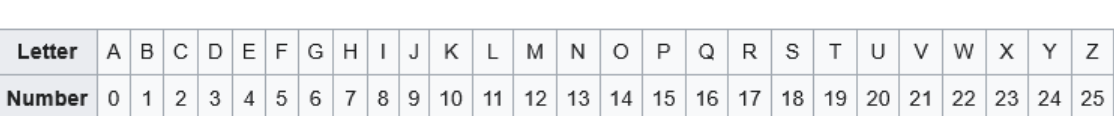
\includegraphics[width=121.80mm,height=31.78mm]{../../images/llm/page_010_img_01.png}%
\end{textblock*}

\end{document}
